% Weight-ceiling proof document — appendix-style standalone (matches thesis preamble
% conventions: 11pt, lmodern, amsthm plain/definition/remark, booktabs, cleveref).
% Source of truth: docs/WEIGHT_CEILING_PROOF.md (v2, 2026-07-10). Oracle-independent.
% Build: pdflatex (TinyTeX) x2.
\documentclass[11pt,a4paper,oneside]{article}
\usepackage[T1]{fontenc}
\usepackage[utf8]{inputenc}
\usepackage{lmodern}
\usepackage{microtype}
\usepackage[a4paper,margin=3cm]{geometry}
\usepackage{amsmath,amssymb,amsthm,mathtools}
\usepackage{graphicx}
\usepackage{booktabs}
\usepackage{enumitem}
\usepackage{xcolor}
\usepackage[hidelinks]{hyperref}
\usepackage[capitalize]{cleveref}
\crefname{conjecture}{Conjecture}{Conjectures}
\Crefname{conjecture}{Conjecture}{Conjectures}

\theoremstyle{plain}
\newtheorem{theorem}{Theorem}[section]
\newtheorem{lemma}[theorem]{Lemma}
\newtheorem{proposition}[theorem]{Proposition}
\newtheorem{corollary}[theorem]{Corollary}
\newtheorem{conjecture}[theorem]{Conjecture}
\theoremstyle{definition}
\newtheorem{definition}[theorem]{Definition}
\theoremstyle{remark}
\newtheorem{remark}[theorem]{Remark}

\DeclareMathOperator{\wt}{wt}
\DeclareMathOperator{\stab}{stab}
\DeclareMathOperator{\Sym}{Sym}
\newcommand{\ZZ}{\mathbb{Z}}
\newcommand{\QQ}{\mathbb{Q}}
\newcommand{\RR}{\mathbb{R}}
\newcommand{\CC}{\mathbb{C}}
\newcommand{\Tcl}{\mathcal{T}}
\newcommand{\zt}[1]{\zeta_{#1}}
\newcommand{\fl}[1]{\left\lfloor #1 \right\rfloor}
\newcommand{\ceilw}{2k + 2\fl{\tfrac{k-1}{3}}}
\newcommand{\pmgw}{2k + 2\fl{\tfrac{k-2}{3}}}
\newcommand{\statOPEN}{\textcolor{red!60!black}{\textsc{open}}}
\newcommand{\statCOND}[1]{\textcolor{orange!70!black}{\textsc{conditional on #1}}}

\title{The weight ceiling for $k$-uniform tilings:\\
$W(k) = 2k + 2\lfloor (k-1)/3\rfloor$\\[1ex]
\large Proof document (appendix draft, oracle-independent)}
\author{A.~Longo \and Claude (CC)\thanks{Extremal construction and the $8/3$ slope
conjecture: A.~Longo. Proof architecture, lemmas, and drafting: CC. Hardened by six
adversarial referee subagents in two rounds; \cref{sec:adversarial} documents the process.
Source of truth: \texttt{docs/WEIGHT\_CEILING\_PROOF.md}, v2, 2026-07-10.}}
\date{July 10, 2026}

\begin{document}
\maketitle

\begin{abstract}
\noindent For edge-to-edge tilings of the plane by unit-edge regular polygons with
$3,4,6,12$ sides, we study $W(T)$, the least possible maximum step-weight of a basis of the
period lattice, as a function of the number $k$ of vertex orbits. We prove, with no
reference to enumeration data: (i) an exact ceiling $W \le \ceilw$ for $k$-uniform tilings
of shortest period length $2$ with symmetry group $pgg$, via a three-constraint integer
program over slab decompositions, together with the matching $pmg$ law $\pmgw$; (ii) a
matching construction schema; (iii) a global upper bound architecture whose remaining gaps
are isolated and stated precisely (\cref{sec:status}). The asymptotic slope is $8/3$, and
$pgg$ is the unique wallpaper group attaining it, with $pmg$ exactly one phase behind. The
ceiling is the \emph{global} maximum only for $k \ge 4$: at $k = 1, 2, 3$ rigid $p6m$
tilings (the $4.6.12$ tiling at $k=1$) reach $k + 4 = 5, 6, 7$, above the $pgg$ line
(\cref{rem:smallk}); a complete all-$k$ budget is $\max(2k+3,\ \ceilw)$. Every decisive
step is either proved here or explicitly ledgered as open; the empirical law that motivated
the theorem (exact on all $\sim$200{,}000 catalogued tilings, $k\le 13$) is used nowhere in
any proof.
\end{abstract}

\section{Setting}\label{sec:setting}

Let $\Tcl$ be the class of edge-to-edge tilings of $\RR^2$ by regular polygons of unit edge
with $3,4,6,12$ sides. (The octagon is excluded: an octagon forces the unique $4.8.8$
tiling, a solved special case; Gr\"unbaum--Shephard \S2.1.) All interior angles are
multiples of $30^\circ$; fixing one edge direction, every edge is parallel to some
$\zt{12}^j$ where $\zt{N} = e^{2\pi i/N}$, and all vertices lie in $x_0 + \ZZ[\zt{12}]
\subset \CC$.

$T$ is \emph{$k$-uniform} if its full symmetry group $G = \Sym(T)$ has exactly $k$ vertex
orbits; such $T$ is crystallographic, so $G$ is a wallpaper group. $\Lambda \subset \CC$
denotes the \emph{full} translation lattice of $G$ (``primitive cell'' always refers to
$\Lambda$; proper-sublattice cells, \emph{supercells}, never enter), $P = G/\Lambda$ the
point group, $|P| \le 12$. With $\stab(v) \le P$ the point stabilizer of a vertex $v$, the
vertex count per primitive cell is
\begin{equation}\label{eq:orbitcount}
n \;=\; \sum_{\text{orbit classes } i} \frac{|P|}{|\stab_i|}.
\end{equation}

For $x \in \ZZ[\zt{24}]$, $\wt(x)$ is the least $m$ with $x$ a sum of $m$ unit
$24$th roots, and
\[
W(T) \;=\; \min_{\text{bases } (u,v) \text{ of } \Lambda} \; \max\bigl(\wt(u), \wt(v)\bigr).
\]
$\wt$ takes positive integer values and any basis witnesses finiteness, so the minimum is
attained. Since $\ZZ[\zt{24}]$ is dense in $\CC$, lower bounds on $\wt$ must be algebraic
(\cref{sec:certificates}), never Euclidean.

\begin{lemma}[$\lambda_1 \ge 1$]\label{lem:lambda1}
Distinct vertices of $T \in \Tcl$ are at distance $\ge 1$; hence every nonzero period has
length $\ge 1$.
\end{lemma}
\begin{proof}
Let $u \ne v$ be vertices with $d(u,v) < 1$. The tiles incident to $v$ cover a neighborhood
of $v$; $u$ is not interior to a tile (no interior vertices) nor to an edge (edge-to-edge),
so $u$ is a corner of a tile incident to $v$; two corners of a unit-edge regular polygon are
at distance $\ge 1$.
\end{proof}

\section{Weight certificates}\label{sec:certificates}

Work in the power basis $e_j = \zt{24}^j$, $j = 0..7$; $\Phi_{24}(x) = x^8 - x^4 + 1$ gives
$\zt{24}^{8+m} = e_{4+m} - e_m$ ($m = 0..3$) and $\zt{24}^{12+j} = -\zt{24}^j$.

\begin{lemma}[certificate principle]\label{lem:certprinciple}
If a $\QQ$-linear functional $\chi$ on $\QQ(\zt{24})$ satisfies $|\chi(\zt{24}^j)| \le 1$
for all $j$, then $\wt(x) \ge |\chi(x)|$ for all $x \in \ZZ[\zt{24}]$.
\end{lemma}

\begin{lemma}[the three certificates]\label{lem:certs}
Let $\varphi(e_4) = 1$, $\psi(e_6) = 1$, $\varphi'(e_0) = 1$ (each vanishing on the other
$e_j$). Then $\varphi, \psi, \varphi + \psi, \varphi'$ all satisfy \cref{lem:certprinciple}
($\varphi + \psi$ because no unit root has both coordinates nonzero). With
$i\sqrt3 = 2e_4 - e_0$ and $i = e_6$:
\begin{enumerate}[label=(\alph*),nosep]
\item for $x = r + c\, i\sqrt3 + s\, i$ with $r$ in the real subfield, $c \in \tfrac12\ZZ$,
$s \in \ZZ$: $\varphi(x) = 2c$, and if moreover $r \in \QQ$ then $\psi(x) = s$, so
$\wt(x) \ge 2c + s$. (The rationality hypothesis is needed because $\psi(\sqrt3) = -1$; on
width-2 tubes all periods have rational real part, \cref{prop:exactweight}.)
\item $\wt(2) = 2$ (via $\varphi'$), and $\wt(c\, i\sqrt3) = 2|c|$ for $c \in \ZZ$ (upper
bound: the two-step word $\zt{12}^2 + \zt{12}^4$).
\end{enumerate}
The real subfield has $\QQ$-basis $\{1,\ 2\cos15^\circ = e_1{+}e_3{-}e_7,\ \sqrt2 =
e_1{+}e_3{-}e_5,\ \sqrt3 = 2e_2{-}e_6\}$, on which $\varphi$ vanishes identically.
(Verified independently by two referees, including all $24$ root values.)
\end{lemma}

\begin{lemma}[tall vectors in every basis]\label{lem:tallvec}
Let $\Lambda = \langle u, v\rangle$ with $u = 2$ and $v = q + iH$, $q \in \QQ$,
$H = c\sqrt3 + s$ ($c, s \in \ZZ_{\ge0}$). Every basis of $\Lambda$ contains a vector $w$
with $\wt(w) \ge 2c + s$.
\end{lemma}
\begin{proof}
$\mathrm{ht} = \operatorname{Im}\colon \Lambda \to \RR$ has image $H\ZZ$; some basis vector
has $|\mathrm{ht}| \ge H$, i.e.\ equals $\pm(q' + i\, mH)$ with $m \ge 1$ and $q' \in \QQ$;
apply \cref{lem:certs}(a).
\end{proof}

\section{Width-2 tubes: structure}\label{sec:structure}

Standing assumptions for \cref{sec:structure,sec:weight,sec:groups,sec:ip}: $T \in \Tcl$
with shortest period $u$, $|u| = 2$.

\begin{lemma}[no oblique width 2]\label{lem:nooblique}
The solutions of $|x|^2 = 4$ in $\ZZ[\zt{12}]$, where for $x = a + b\zt{12} + c\zt{12}^2 +
d\zt{12}^3$
\[
|x|^2 = (a^2{+}b^2{+}c^2{+}d^2{+}ac{+}bd) + \sqrt3\,(ab{+}bc{+}cd),
\]
are exactly the twelve $x = 2\zt{12}^j$. Hence $u$ is parallel to an edge direction; rotate
by a multiple of $30^\circ$ (a symmetry of the direction set and of $\wt$) so that $u = 2$,
and view $T$ on the cylinder $\mathcal{C} = \RR^2/2\ZZ$. (Bounded exhaustive check; run
independently by a referee.)
\end{lemma}

\begin{lemma}[width-2 tile inventory]\label{lem:inventory}
On $\mathcal{C}$ every tile is one of: upright triangle (one horizontal edge), upright
square, or hexagon with horizontal long diagonal spanning the full circumference.
\end{lemma}
\begin{proof}[Proof (by excluded candidate)]
\emph{(a) Dodecagon:} minimal width $2 + \sqrt3 > 2$ in every direction. \emph{(b)
$45^\circ$ square:} not direction-legal ($45^\circ \notin 30^\circ\ZZ$). \emph{(c) Hexagon
with vertical long diagonal} (width $\sqrt3$ across flats): its unit vertical edges leave a
residual column of width $2 - \sqrt3 \approx 0.268$ closing the circumference; any tile
sharing a full unit vertical edge extends $\ge \sqrt3/2 > 0.268$ from it and overlaps
(T-vertices excluded by edge-to-edge), and no tile fits the gap. The same argument excludes
any width decomposition with a residual gap in $(0, \sqrt3/2)$. \emph{(d) Vertical-edge
(``sideways'') triangle and $30^\circ$-tilted square:} \statOPEN\ --- \cref{gap:31d}. \emph{(e)}
These are all direction-legal orientation classes of the four tiles.
\end{proof}

\begin{remark}[Gap 3.1(d)]\label{gap:31d}
The v1 chord-sum exclusion of case (d) was unsound (a referee showed it would also exclude
the surviving hexagon). Two candidate repair routes, neither completed: (i) the
vertex-level affine-chord Diophantine argument (crossing abscissae lie in $\tfrac12\ZZ +
\tfrac{\sqrt3}{6}\ZZ$; a finite case check over crossed-tile sequences with chord sum $2$
remains); (ii) vertical-strip decomposition, where applicable: column widths obey
$m\cdot\tfrac{\sqrt3}{2} + n\cdot 1 + h\sqrt3 = 2$, forcing $m = h = 0$ by irrationality.
Everything in \cref{sec:weight,sec:groups,sec:ip} is conditional on this single point and on
nothing else. The construction of \cref{thm:B} does \emph{not} depend on it: an exhibited
tiling is verified directly.
\end{remark}

\begin{lemma}[slab decomposition]\label{lem:slabs}
Granting \cref{lem:inventory}, $\mathcal{C}$ splits into a cyclic stack of slabs:
\emph{(T)} triangle slab, height $\sqrt3/2$, one up- and one down-triangle per cell,
$2$ vertices; \emph{(S)} square slab, height $1$, exactly two unit squares, $2$ vertices;
\emph{(H)} hexagon slab, height $\sqrt3$, one full-width hexagon plus two corner triangles,
$3$ vertices. (Each slab is charged the vertices of its lower boundary row; cyclically every
vertex is charged once.)
\end{lemma}
\begin{proof}
Only squares have vertical edges; a square's vertical edge must abut, full length, another
square's (edge-to-edge, no T-vertices), so squares propagate into a full ring of two: type
(S). A hexagon's horizontal long diagonal has length $2$, the full circumference, so its
endpoints coincide on $\mathcal{C}$: one hexagon per H slab, corners filled by one triangle
above and one below (areas: $2\sqrt3 = \tfrac{3\sqrt3}{2} + 2\cdot\tfrac{\sqrt3}{4}$). The
rest is rows of upright triangles: type (T).
\end{proof}

Erasing S slabs, the T/H stack is the triangular row grid (rows at spacing $\sqrt3/2$, two
vertices per row per cell, $x$-offsets alternating $\{0,1\}$ and $\{\tfrac12,\tfrac32\}$
mod $2$) minus a set $D$ of deleted vertices (hexagon centers), one per H slab.

\begin{lemma}[deletion cascade]\label{lem:cascade}
If $(x, \text{row } j) \in D$ then no other vertex of rows $j{-}1, j, j{+}1$ is in $D$.
Consequently deletions occupy pairwise non-adjacent rows.
\end{lemma}
\begin{proof}
Two hexagons cannot share a triangle. Same row: the partner vertex is at distance $1$.
Adjacent rows: both vertices are at displacement $(\pm\tfrac12, \pm\tfrac{\sqrt3}{2})$ ---
using $x \pm \tfrac32 \equiv x \mp \tfrac12 \pmod 2$ --- distance exactly $1$ (minimum over
lifts).
\end{proof}

\section{The exact weight of a width-2 tube}\label{sec:weight}

Let the primitive cell consist of $a$ H slabs, $t$ T slabs, $s$ S slabs, so the cell height
is $H = a\sqrt3 + t\tfrac{\sqrt3}{2} + s$ and
\begin{equation}\label{eq:vertexcount}
n = 3a + 2t + 2s.
\end{equation}

\begin{lemma}[slab path; zero splices]\label{lem:slabpath}
There is an edge path from a vertex $x$ to $x + v$ ($v$ the tall period) of length exactly
$2a + t + s$.
\end{lemma}
\begin{proof}
Monotone per-slab chains: T $=$ one $60^\circ$ edge (gain $\sqrt3/2$, entry at either slot,
exit shift $\pm\tfrac12$ with free sign); S $=$ one vertical edge (gain $1$, shift $0$);
H $=$ two edges up a hexagon flank through the full-width vertex (the two long-diagonal
endpoints are one point on $\mathcal{C}$), gain $\sqrt3$, entering at \emph{either} slot of
the lower boundary row and exiting directly above the entry. Since H slabs accept either
entry slot, consecutive chains splice with no extra edges for every deletion word; the
T-slab signs realize any net shift of the correct parity, matching the real part $q$ of $v$.
Total: $2a + t + s$ edges.
\end{proof}

\begin{proposition}[exact weight]\label{prop:exactweight}
Vertex $x$-coordinates lie in $\tfrac12\ZZ$, so all periods have rational real part, and
\[
\wt(v) = 2a + t + s, \qquad
W(T) = \max(2,\, 2a + t + s).
\]
\end{proposition}
\begin{proof}
Upper: \cref{lem:slabpath}. Lower: $\operatorname{Im} v = \tfrac{2a+t}{2}\sqrt3 + s$;
\cref{lem:certs}(a) with $c = \tfrac{2a+t}{2} \in \tfrac12\ZZ$ gives $\wt(v) \ge 2a + t +
s$; every basis contains a vector of $|\mathrm{ht}| \ge H$ (\cref{lem:tallvec}) with the
same bound, and $\wt(u) = 2$.
\end{proof}

Writing $b$ for the number of orbit classes with $|\stab| = 2$ and granting $\stab \le 2$
for the relevant groups (\cref{lem:stab}), \cref{eq:orbitcount} gives $n = 4k - 2b$, hence
by \cref{eq:vertexcount}
\begin{equation}\label{eq:master}
\wt(v) \;=\; 2a + t + s \;=\; \frac{n + a}{2} \;=\; 2k - b + \frac{a}{2}.
\end{equation}
Everything now rides on capping $a$ (the hexagon count) via the group.

\section{Groups on width-2 tubes}\label{sec:groups}

\begin{lemma}[rigid groups cap at $k \le 4$, $W = 2$]\label{lem:rigid}
If $P$ contains a rotation of order $3, 4, 6$, the lattice is hexagonal or square, so
$\lambda_2 = \lambda_1 = 2$ and the cell area is $2\sqrt3$ or $4$. The minimal vertex
corner-area is $a_{\min} = \sqrt3/2$ (the $3^6$ vertex), so $n \le 4$, $k \le 4$, and both
periods have weight $2$: $W = 2 < \ceilw$ for $k \ge 2$. (Boundary example: the kagome
tiling --- width 2, $p6m$, $k = 1$, $n = 3$.)
\end{lemma}

\begin{lemma}[vertical mirrors]\label{lem:vmirror}
If $G$ contains a reflection with vertical axis, its two axis lines pin one offset class of
rows pointwise, and every deletion row is pinned-parity (a deletion in a swapped row would
force a second, adjacent deletion). Accounting: pinned vertices $\ge a$, so with $|P| = 4$,
$k \ge (n + a)/4 = \wt(v)/2$, i.e.\ $W \le 2k$; with $|P| = 2$ (pm, cm), $W \le k$.
\end{lemma}

\begin{lemma}[single-parity deletions force a mirror]\label{lem:parity-mirror}
The two vertical-mirror classes on $\mathcal{C}$ are $x \mapsto -x$ (fixes integer offsets
pointwise, swaps half-integer ones) and $x \mapsto 1 - x$ (vice versa); both preserve the
triangular grid and all S slabs. If all deletions sit at integer offsets, $x \mapsto -x$ is
a symmetry of $T$; if all at half-integer offsets, $x \mapsto 1 - x$ is. (A width-2 tube of
this class is determined by its deletion set and S-slab positions, so a grid isometry
preserving $D$ is a symmetry --- the \emph{determined-by-word principle}.)
\end{lemma}

\begin{lemma}[stabilizers for $pgg$ and $pmg$]\label{lem:stab}
$pgg$ has no reflections; its non-translations are glides and $2$-folds, so vertex
stabilizers have order $\le 2$. The same holds for $pmg$: an order-4 stabilizer inside
$2mm$ would put a $2$-fold on a mirror axis, whose product with the mirror is the
perpendicular reflection through that point, giving two mirror directions (pmm or cmm).
Hence $c = 0$ in \cref{eq:orbitcount}, $n = 4k - 2b$ is even, and $a$ is even.
\end{lemma}

\begin{lemma}[cmm centering]\label{lem:cmm}
For cmm the primitive cell is spanned by $u = 2$ and a centering vector $(q, H/2)$ with $q$
odd; the accounting of \cref{lem:vmirror} applied to the centered cell gives $W \le 2k$ for
every cmm width-2 tube.
\end{lemma}

\section{The integer program and the exact laws}\label{sec:ip}

Standing: width-2 tube, granting \cref{gap:31d}; slab data $(a, t, s)$, $b$ pinned orbit
classes, $\wt(v) = 2k - b + \alpha$ with $\alpha = a/2 \in \ZZ$ (\cref{lem:stab}).

\begin{lemma}[the three constraints]\label{lem:constraints}
For a primitive width-2 tube with $G = pgg$ (and, where noted, $pmg$ --- both contain the
vertical-axis glide family):
\begin{enumerate}[label=(\roman*),nosep]
\item[(iii)] \emph{Integral, even shear.} $q \in \ZZ$: $q \in \tfrac12\ZZ$ by
\cref{sec:structure}, and $\Lambda$ is invariant under the point-group reflection
$x \mapsto -x$, so $(2q, 0) \in \Lambda \cap \RR = 2\ZZ$. $q$ even: if $q$ were odd, the
vertical translations in $\Lambda$ are $2H\ZZ$ and $\gamma^2 = (0, 2\delta) \in \Lambda$
gives $\delta \equiv 0$ or $H \pmod{2H}$; $\delta \equiv 0$ makes $\gamma$ a vertical
mirror modulo $\Lambda$, and $\delta \equiv H$ makes $t_{-v}\circ\gamma$ a vertical mirror
outright --- both absent in $pgg$ (and in $pmg$, else pmm/cmm). So $q$ is even and
$\Lambda = \langle(2,0),(0,H)\rangle$.
\item[(i)] \emph{Even counts.} $\gamma^2 = (0, 2\delta) \in H\ZZ$ gives $\delta \in \{0,
H/2\}$; $\delta = 0$ is a mirror, so $\delta = H/2$. $\gamma$ shifts the slab stack by
$H/2$ and no slab is $\gamma$-invariant (its lower boundary height would satisfy $\beta +
H/2 \equiv \beta \pmod H$), so the shift pairs slabs type-preservingly: $a, t, s$ are all
even.
\item[(ii)] \emph{Mirror exclusion.} If $a > 0$, deletions occur at both offset parities
(else \cref{lem:parity-mirror} contradicts $pgg$). Offset parity switches exactly across
each T slab and is preserved by H and S slabs; $t$ is even by (i) and the switches around
the cycle number $\ge 2$, in $\ge 2$ odd T-runs: $t \ge 2$.
\end{enumerate}
Moreover $t + s = 2k - b - 3\alpha$, and $t, s$ even forces $b \equiv \alpha \pmod 2$.
\end{lemma}

\begin{theorem}[width-2 $pgg$ law; conditional only on \cref{gap:31d}]\label{thm:A}
For every $k \ge 2$, every primitive $k$-uniform width-2 tube with $G = pgg$ satisfies
\[
W \;\le\; \ceilw,
\]
and the bound is attained (\cref{thm:B}).
\end{theorem}
\begin{proof}
$W = 2k - b + \alpha$ by \cref{eq:master}. If $a = 0$: $W \le 2k - b \le 2k$. If $a > 0$:
$t \ge 2$ gives $3\alpha \le 2k - b - 2$, so $\alpha - b \le (2k - 2 - 4b)/3 \le (2k-2)/3$;
$\alpha - b$ is an even integer, so
\[
\alpha - b \;\le\; 2\fl{\tfrac{1}{2}\fl{\tfrac{2k-2}{3}}} \;=\; 2\fl{\tfrac{k-1}{3}}
\]
(residues: $k = 3m \Rightarrow \fl{(6m-2)/3} = 2m{-}1 \to 2m{-}2$; $k = 3m{+}1 \Rightarrow
2m$; $k = 3m{+}2 \Rightarrow 2m$), and the $b > 0$ branches never exceed the $b = 0$ value.
\end{proof}

\begin{remark}[v1's error, for the record]\label{rem:v1}
Version 1 claimed the extremum on pure hexagon/triangle tubes (``squares only dilute'').
False: at $k \not\equiv 1 \pmod 3$ the maximum requires S slabs, and v1's extremal family
was mirror-symmetric, hence $pmg$, not $pgg$. Both errors were found in the adversarial
round (and the first independently by the author); the program above supersedes that
treatment and explains why catalogued non-jump-$k$ extremals contain squares.
\end{remark}

\begin{theorem}[width-2 $pmg$ law; same conditionality]\label{thm:C}
For $pmg$ (mirrors necessarily horizontal on an extremal tube, since vertical mirrors give
$W \le 2k$): $W \le \pmgw$. Attainment: Appendix~A.2, \statOPEN.
\end{theorem}
\begin{proof}[Proof sketch]
$pmg$'s two horizontal mirror-axis classes must each be \emph{hosted}: on a vertex row or a
hexagon-center row (pinning: $b \ge 1$), or on an S-slab midline (no pinning, but then
$s \ge 2$ by even counts). The trichotomy is exhaustive: a mid-T or quarter-H axis swaps
rows of opposite offset parity while preserving $x$ --- impossible; oblique mirrors would
map $u$ to another length-2 period and die by \cref{lem:nooblique} plus $H > \sqrt3$.
With $t \ge 2$ (no vertical mirrors, else pmm) the two branches give:
$s$-hosted, $3\alpha \le 2k - b - 4$, so $\alpha - b \le 2\fl{(k-2)/3}$; vertex-hosted,
$b \ge 1$ and $\alpha - b \le (2k - 2 - 4b)/3$, whose even-floor at $b = 1$ \emph{equals}
$2\fl{(k-2)/3}$ at $k \equiv 0, 1 \pmod 3$ and is strictly smaller otherwise; $b \ge 2$ is
strictly smaller everywhere. Never exceeded.
\end{proof}

\begin{theorem}[achievability --- construction schema]\label{thm:B}
For every $k \ge 2$ there is a $k$-uniform $F(k) \in \Tcl$ with $\Sym(F(k)) = pgg$ exactly
and $W(F(k)) = \ceilw$.
\end{theorem}
\begin{proof}[Construction schema; explicit words: Appendix A.1, \statOPEN]
Take $\alpha^\ast = 2\fl{(k-1)/3}$, $a = 2\alpha^\ast$, $t + s = 2k - 3\alpha^\ast$ with
$t \ge 2$, all counts even, $t$ split into two odd runs placed asymmetrically. Deletion
offsets: a half-word $w$ on the lower half-cell's hexagon slots, the upper half its
$\gamma$-image (offset-flipped, shifted $H/2$); the two odd T-runs put the halves at
opposite offset parities, breaking both vertical mirrors (\cref{lem:parity-mirror}); a
single defect in $w$ kills every vertical sub-translation and every horizontal mirror; the
$2$-fold centers land at hexagon centers and edge midpoints ($b = 0$). Verification duties,
each finite and mechanical per $k$: cascade-legality; $G \supseteq pgg$; no mirror and no
proper sub-period ($G = pgg$ on the claimed cell); $b = 0$, so $k(F) = n/4 = k$;
$W = 2k + \alpha^\ast$ by \cref{prop:exactweight}. $\Sym(F)$ can exceed $pgg$ only via
mirrors, higher rotations (excluded: rectangular lattice, $\lambda_1 = 2 \ne \lambda_2$),
or extra translations --- each excluded.
\end{proof}

\section{The global upper bound and Lemma M}\label{sec:global}

Gauss-reduced $\lambda_1 \le \lambda_2$, angle in $[60^\circ, 90^\circ]$;
$A = |\det\Lambda| \le a_{\max}|P|k$ with $a_{\max} = \tfrac{\sqrt3}{12} +
2\cdot\tfrac{2+\sqrt3}{4} \approx 2.011$ (the $3.12.12$ vertex).

\begin{lemma}[crossing bound; crude constant proven, sharp constant open]\label{lem:crossing}
For any $T \in \Tcl$ and period $x$: $\wt(x) \le c_1|x| + c_2$ with $(c_1, c_2) =
(94, 136)$. \emph{(Referee-supplied proof: perturb the segment off all vertices; vertices
are $1$-separated (\cref{lem:lambda1}), so $\le 2.6|x| + 3.6$ of them lie within $1/2$ of
the segment; each contributes $\le 6$ crossed incident edges; each crossed tile costs
$\le 6$ boundary edges.)} Appendix~B's target is $c_1 \le 2 + \varepsilon$ via band
decomposition; everything below keeps $c_1$ symbolic.
\end{lemma}

\begin{lemma}[width-1 automatic mirror]\label{lem:width1}
A width-1 tube has all tiles upright triangles/squares, one vertex per row, all in one
coset $\{x_0, x_0 + \tfrac12\}$ of $\tfrac12\ZZ$; the reflection $x \mapsto 2x_0 - x$ fixes
both cosets and every slab, so $G$ contains a vertical mirror with every vertex on an axis:
$n \le 2k$ and $W \le 2k$.
\end{lemma}

\textbf{Case W1 (rigid lattices).} $\lambda_2 = \lambda_1$: $W \le c_1\sqrt{2A/\sqrt3} +
c_2 = O(\sqrt k)$, below the ceiling for $k \ge 34$ when $c_1 = 2$; small cells have
bounded $k$ by the corner-area count (\cref{lem:rigid} handles $\lambda_1 = 2$).

\textbf{Case W2 (wide).} For $\lambda_1 \ge T_0 := c_1\, a_{\max} |P| \tfrac{2}{\sqrt3}
\cdot \tfrac38$ with $|P| \le 4$: $W \le c_1\lambda_2 + c_2 \le \tfrac83 k + c_2$. This
yields the \emph{slope}, not the exact floor form; $T_0 = 7$ if $c_1 = 2$ is proven,
$T_0 \approx 330$ under the crude constant.

\textbf{Case W3.} $\lambda_1 \in \{1, 2\}$: \cref{lem:width1} and
\cref{sec:structure,sec:weight,sec:groups,sec:ip}.

\begin{remark}[small-$k$ scope; the rigid regime dominates for $k \le 3$]\label{rem:smallk}
The $pgg$ ceiling is the global maximum only for $k \ge 4$. At $k = 1, 2, 3$ the maximum
weight is $k + 4$ (values $5, 6, 7$), achieved by rigid $p6m$ tilings: $4.6.12$ at $k = 1$,
the $3.4.6.12$ family at $k = 2, 3$. No theorem here is contradicted --- Case~W1 bounds the
rigid regime by $O(\sqrt k) + \mathrm{const}$, which dominates at small $k$ --- but the
headline requires the qualifier, and a provably complete all-$k$ enumeration budget is
$\max(2k + 3,\ \ceilw)$, the first term binding only for $k \le 3$ and tight only at
$k = 1$. Exactness of the three small-$k$ values is a finite verification (rigid lattice
with $k \le 3$ bounds the cell area, hence the candidate tilings), \statOPEN. The mechanism
(A.L.) is an escape-cost model: on round lattices $W \approx 2c + \mathrm{traverse} + O(1)$,
where $c \le 2$ is the cost of escaping a $12$-gon vertex and the traverse term is the
orbit-graph diameter, $O(\sqrt k)$ for compact fundamental domains. The model is intended for (and correct in) the rigid regime only; its middle term relies on
orbit-graph connectivity of the fundamental domain, which holds for compact domains but
fails in the stretched $pgg$ regime --- which is why the two regimes need the two different
arguments of this document. Extrapolated outside its regime, $2c + 2k - 1 = 2k + 3$ would
first be overtaken by the $pgg$ ceiling at $k = 7$ ($17 < 18$): one way to locate the
regime boundary.
\end{remark}

\begin{conjecture}[Lemma M --- the residual band, \statOPEN]\label{conj:M}
For every $k$-uniform $T \in \Tcl$ with $\lambda_1 \in (1,2) \cup (2, T_0)$:
$W(T) \le \ceilw$.
\end{conjecture}

\begin{remark}[scope of \cref{conj:M}, from the adversarial round]
(i) The band must be binned by $(|\lambda_1|^2, \text{angle})$ class: off-axis shortest
periods exist at many norms (e.g.\ $1 + \zt{12}$, length $2\cos 15^\circ \approx 1.93$,
$15^\circ$ off-axis), and the slab machinery does not apply to them as-is. (ii) The
strongest counterexample attempt so far --- a genuine width-$(1{+}\sqrt3)$ hexagon+square
strip, verified to exist, $3$-uniform --- has $W/k = 1$: its forced mirrors destroy the
economy, evidence \emph{for} the conjecture. (iii) No construction beating slope $8/3$ was
found.
\end{remark}

\section{The group ledger}\label{sec:ledger}

\begin{table}[h]\centering
\begin{tabular}{@{}lll@{}}
\toprule
group(s) & mechanism & width-2 result \\
\midrule
$p3, p3m1, p31m, p6, p6m, p4, p4m, p4g$ & rigid lattice (\cref{lem:rigid}) & $k \le 4$, $W = 2$ \\
$p1$ & $|P| = 1$: $n = k$, $a \le k/3$ & $W \le \tfrac23 k$ \\
$p2, pg$ & $|P| = 2$, no mirrors: $n \le 2k$ & $W \le \tfrac43 k$ \\
$pm, cm$ & $|P| = 2$, mirrors (\cref{lem:vmirror}) & $W \le k$ \\
$pmm, cmm$ & mirrors both directions (\cref{lem:vmirror,lem:cmm}) & $W \le 2k$ \\
$pmg$ & mirror hosting (\cref{thm:C}) & $\pmgw$ \\
$pgg$ & \cref{thm:A,thm:B} & $\boldsymbol{\ceilw}$ \\
\bottomrule
\end{tabular}
\caption{Width-2 ceilings per wallpaper group. Among tube-capable groups, $pgg$ maximizes
(steps per vertex) $\times$ (orbit size): its point group has order $4$ while its only
constraint costs the additive minimum ($t \ge 2$); mirror groups pay multiplicatively
(pinned rows), $|P| = 2$ groups halve the multiplier, rigid groups cannot form tubes.
$pgg$'s own 2-fold centers make the bound $\ceilw$ rather than $\tfrac83 k$: the parity
link of \cref{lem:constraints} is where they bite. $pmg$ trails by one phase because its
mirrors must be hosted.}
\end{table}

\begin{figure}[h]\centering
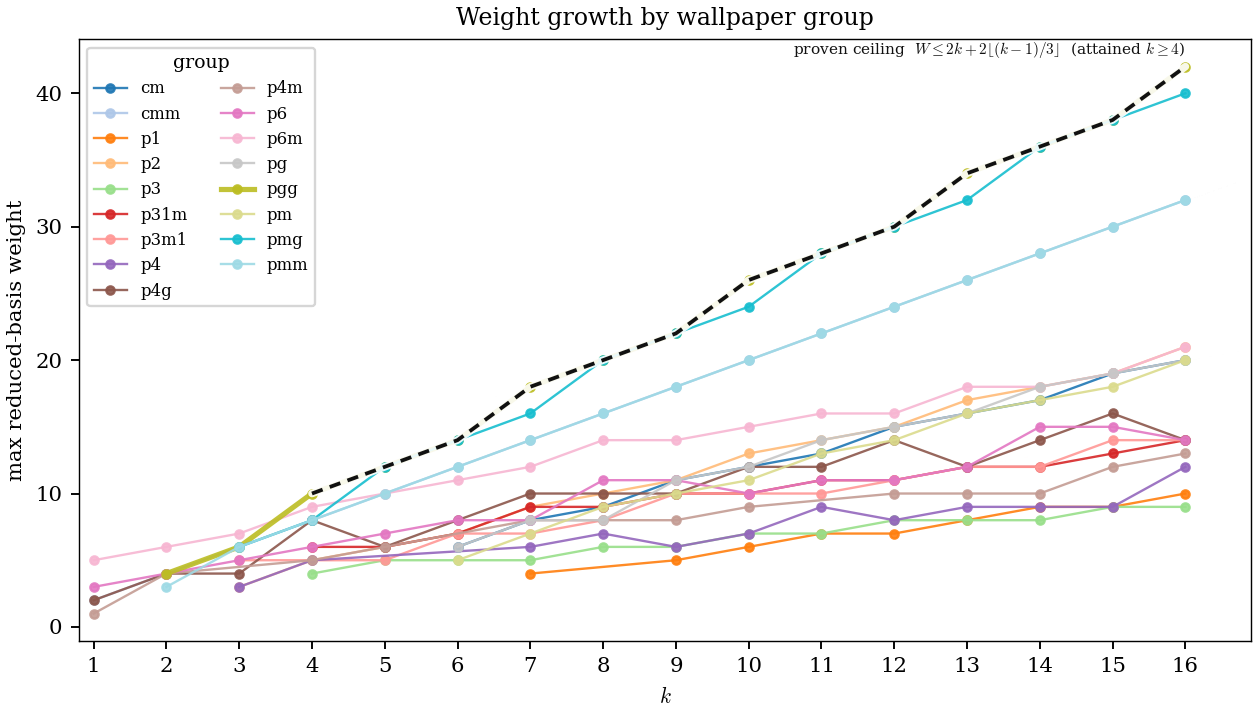
\includegraphics[width=0.92\textwidth]{ctrnact-weight-by-group.png}
\caption{Empirical consistency (no proof role): measured maximum reduced-basis weight per
wallpaper group, $k \le 11$ catalogue. The proven $pgg$/$pmg$ laws match every point; the
extension runs at $k = 12, 13$ (maxima $30$ and $34$, the predicted jump to $2k+8$)
likewise. The theorems above were derived and verified without reference to this data.}
\end{figure}

\section{Status ledger}\label{sec:status}

\noindent\textbf{Proven unconditionally:} \cref{sec:setting,sec:certificates} (certificates
independently verified twice); \cref{lem:nooblique}; \cref{lem:inventory}(a)(b)(c)(e);
\cref{lem:slabs,lem:cascade,lem:slabpath}; \cref{prop:exactweight};
\cref{lem:rigid,lem:vmirror,lem:parity-mirror,lem:stab,lem:cmm,lem:constraints};
\cref{thm:A,thm:C} modulo \cref{gap:31d}; \cref{thm:B} modulo the finite Appendix-A
verifications; \cref{lem:crossing} (crude); \cref{lem:width1}; Cases W1--W3.

\smallskip
\noindent\textbf{Open:} \cref{gap:31d} (width-2 tilted-tile exclusion; isolated, two
candidate routes); \cref{conj:M} (residual widths, binned by norm and angle); Appendix~A
(explicit deletion words; finite, mechanical); Appendix~B (sharp crossing constant, which
sets $T_0 \in \{7, \dots, {\sim}330\}$); the finite small-$k$ rigid verification of
\cref{rem:smallk} ($k \le 3$ maxima $= k + 4$).

\smallskip
\noindent\textbf{Not claimed:} the exact law on the wide regime; anything about star or
non-unit polygons or octagon-bearing tilings.

\smallskip
\noindent\textbf{Addendum (2026-07-10, post-publication of this ledger).} (i) The small-$k$
verification is DONE and refereed: the companion appendix \emph{Exact weight maxima at
$k \le 3$} proves $\max W = 5, 6, 7$ exactly, discharging the last Open item above.
(ii) \cref{gap:31d} has been identified with the independently-discovered obligation
E4-A$'$ of the TH-10 band program: one finite exclusion now gates all $378$ catalogued
$\lambda_1 = 2$ tilings AND the conditionality of \cref{thm:A,thm:C}; a slab-engine
computation (reachable-closure increment already reproduces the $\{T,S,H\}$ inventory
mechanically) is the designated closer. (iii) Progress on \cref{conj:M}: the bands
$\lambda_1 = 1$ and $\lambda_1 = \sqrt3$ (hexagon-bearing) are now CLOSED against the
ceiling for all $k \ge 4$, at $W(\Lambda) \le 2k$ each, by refereed exact layered-word
climbs (consolidation note, 2026-07-10); the snub band $\lambda_1 = 2\cos 15^\circ$ is
re-scoped (weak climbing chains are real; a row-word classification is the route). The
program's dependency structure lives in \texttt{docs/WEIGHT\_PROOF\_DAG.md} and the
DAG-status appendix.

\section{The adversarial round (documentation)}\label{sec:adversarial}

Five independent referee subagents attacked v1 (2026-07-10): algebra/parity, width-2
geometry, group theory, global-bound/counterexamples, and global soundness; a sixth then
attacked the rebuilt core (\cref{sec:weight,sec:ip}, \cref{thm:C}). Score: the
\cref{sec:certificates} certificates were verified in full twice. Fatal findings, all
repaired: v1's extremal family was mirror-symmetric ($pmg$, not $pgg$; found independently
by the author); v1's key lemma composed a glide with a rotation into a ``translation''
(impossible by orientation; replaced by the determined-by-word argument of
\cref{lem:parity-mirror}); v1's tile-inventory proof was self-refuting (it excluded its own
hexagon; rebuilt, case (d) honestly re-opened); ``squares only dilute'' was false
(\cref{rem:v1}); the $pmg$ corollary was wrong as argued (rebuilt as \cref{thm:C}).
The final round found no fatal errors and re-derived both exact formulas by independent
brute force over the constraint system at $k = 2..13$ with no mismatches.

\end{document}
